% Title: gl2ps_renderer figure
% Creator: GL2PS 1.4.2, (C) 1999-2020 C. Geuzaine
% For: Octave
% CreationDate: Tue Oct 26 15:49:43 2021
\setlength{\unitlength}{1pt}
\begin{picture}(0,0)
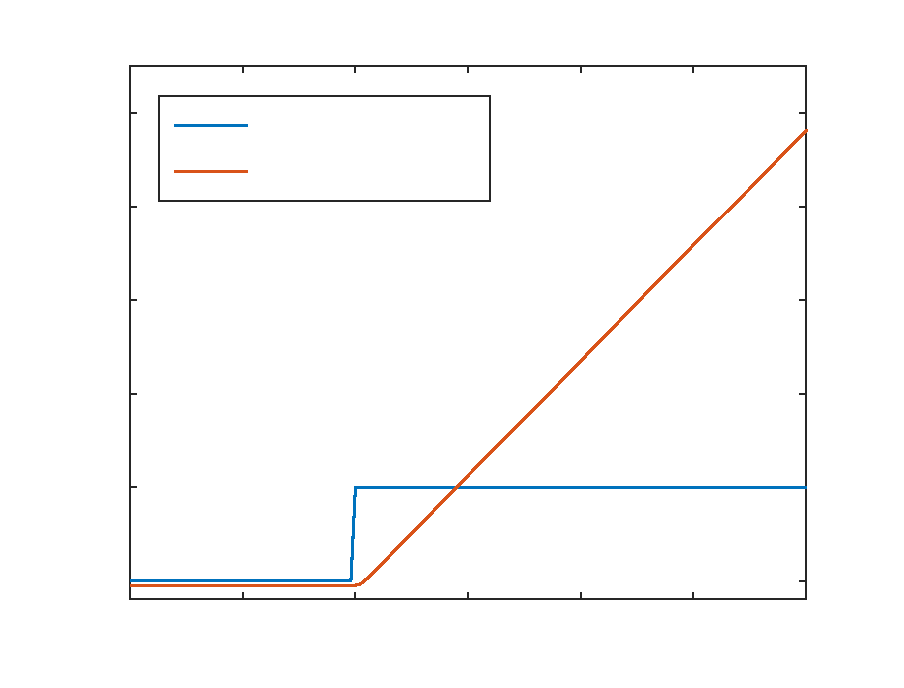
\includegraphics[scale=1]{motorDC1-inc}
\end{picture}%
\begin{picture}(418,314)(0,0)
\fontsize{10}{0}\selectfont\put(54.4343,27.0024){\makebox(0,0)[t]{\textcolor[rgb]{0.15,0.15,0.15}{{0}}}}
\fontsize{10}{0}\selectfont\put(108.52,27.0024){\makebox(0,0)[t]{\textcolor[rgb]{0.15,0.15,0.15}{{0.5}}}}
\fontsize{10}{0}\selectfont\put(162.605,27.0024){\makebox(0,0)[t]{\textcolor[rgb]{0.15,0.15,0.15}{{1}}}}
\fontsize{10}{0}\selectfont\put(216.69,27.0024){\makebox(0,0)[t]{\textcolor[rgb]{0.15,0.15,0.15}{{1.5}}}}
\fontsize{10}{0}\selectfont\put(270.776,27.0024){\makebox(0,0)[t]{\textcolor[rgb]{0.15,0.15,0.15}{{2}}}}
\fontsize{10}{0}\selectfont\put(324.861,27.0024){\makebox(0,0)[t]{\textcolor[rgb]{0.15,0.15,0.15}{{2.5}}}}
\fontsize{10}{0}\selectfont\put(378.946,27.0024){\makebox(0,0)[t]{\textcolor[rgb]{0.15,0.15,0.15}{{3}}}}
\fontsize{10}{0}\selectfont\put(49.4418,43.4814){\makebox(0,0)[r]{\textcolor[rgb]{0.15,0.15,0.15}{{0}}}}
\fontsize{10}{0}\selectfont\put(49.4418,88.3842){\makebox(0,0)[r]{\textcolor[rgb]{0.15,0.15,0.15}{{1}}}}
\fontsize{10}{0}\selectfont\put(49.4418,133.287){\makebox(0,0)[r]{\textcolor[rgb]{0.15,0.15,0.15}{{2}}}}
\fontsize{10}{0}\selectfont\put(49.4418,178.19){\makebox(0,0)[r]{\textcolor[rgb]{0.15,0.15,0.15}{{3}}}}
\fontsize{10}{0}\selectfont\put(49.4418,223.093){\makebox(0,0)[r]{\textcolor[rgb]{0.15,0.15,0.15}{{4}}}}
\fontsize{10}{0}\selectfont\put(49.4418,267.995){\makebox(0,0)[r]{\textcolor[rgb]{0.15,0.15,0.15}{{5}}}}
\fontsize{11}{0}\selectfont\put(216.69,14.0024){\makebox(0,0)[t]{\textcolor[rgb]{0.15,0.15,0.15}{{Tempo (s)}}}}
\fontsize{11}{0}\selectfont\put(38.4418,162.474){\rotatebox{90}{\makebox(0,0)[b]{\textcolor[rgb]{0.15,0.15,0.15}{{Tensão (V)}}}}}
\fontsize{9}{0}\selectfont\put(117.934,261.872){\makebox(0,0)[l]{\textcolor[rgb]{0,0,0}{{Tensão de entrada}}}}
\fontsize{9}{0}\selectfont\put(117.934,239.999){\makebox(0,0)[l]{\textcolor[rgb]{0,0,0}{{Tensão no potenciómetro}}}}
\end{picture}
